\chapter{Kinetic model of NER}
\label{chap:kineticNERmodel}

Luijsterburg \textit{et al.} developed a mathematical NER model by integrating a large dataset for all seven core NER factors \cite{Luijsterburg2010}. However, despite the comprehensive collection of time-resolved \textit{in vivo} measurements of the individual protein dynamics the model parameters comprising binding, dissociation and catalytic constants were not fully identified by the data. This is presumably caused by the missing readout of DNA repair, which was so far not measured on a similar time-scale as the protein assembly rates and the dwell times. Unfortunately, the non-identifiability sets a limitation for the predictive power of the model. \\ 
Based on the EdU incorporation data introduced in chapter \ref{chap:quantData} we present here an evolved mathematical model of NER that explains the connection between the dynamic exchange of individual repair factors at damaged chromatin sites and the overall time scale of the entire repair process. We calibrate the parametrization of the model iteratively with a profile likelihood estimation leading to identifiable parameters and hence an increased predictive power of the model. As a consequence, our fully identifiable model can reliably predict the behaviour of the experimentally inaccessible repair intermediate of incised DNA.\\
   



\section{Slow first-order reaction kinetic due to many fast interacting components}
\label{sec:toyModel}
To investigate the mechanistic connection between fast NER factor exchange at the DNA template and the overall slow repair time, it appears practical to apply an analytical approach. During her Ph.D. thesis, Dr.\ Gesa Terstiege supervised by Prof.\ Thomas H\"ofer performed this analysis \cite{Terstiege2010,Verbruggen2014}, considering the complex formation with a simplified model of repair including $N$ repair factors. They examined different scenarios distinguishing between random and sequential protein assembly; reversible and irreversible protein binding, or mixed mechanisms specific for each DNA repair intermediate (\textit{cf.}\ Figure \ref{fig:reactionTiming}A,\cite{Verbruggen2014}). Under appropriate assumptions, the mean repair time of such a complex assembly process can be generally described with:

\begin{equation}
\tau = \underbrace{\frac{1}{k}\sum^{N-1}_{i=0}K_i\left(\frac{l}{k}\right)^i}_{\text{first assembly}} +  \underbrace{\frac{1}{\rho}\sum_{i=0}^{N}J_i \left(\frac{l}{k}\right)^i}_{\text{reassembly and reaction}}, \label{Eqn:taugen}
\end{equation}

where $k$ denotes the pseudo first-order association rate constant of NER factors, $l$ the dissociation rate constant of NER factors and $\rho$ the rate of the repair reaction. $K_i$ and $J_i$ differ between random assembly
\begin{equation}
K_i^\text{rand}= \sum_{j=1}^{N-i}\frac{1}{i+j}\frac{{N \choose j-1}}{{N\choose i+j}} , \quad J_i^\text{rand} = {N\choose i}\label{Eqn:coefrand}
\end{equation} 
and sequential assembly           
\begin{equation}
K_i^\text{seq}= N-i , \quad J_i^\text{seq} = 1.\label{Eqn.coefseq}
\end{equation}
Considering reversible protein binding ($l=k=1$), sequential and random assembly occur on a similar time scale for fewer than or equal to 10 components \cite{Terstiege2010}, which coincides with the number of core NER factors \cite{Luijsterburg2010}. The theoretical component number where both assembly strategies have a similar timing is even higher for increasing reaction rates ($\rho \gg k,l$). Given that all repair factor dwell times are in the order of $\sim$1 min ($k$ = $l$ = 1 $\text{min}^{-\text{1}}$), the model was simulated for $N$ = 9 components. The resulting trajectory followed a single-exponential kinetic with a half-time of $\sim$1 hour in the case of balanced reversibility. In contrast, for an irreversible process ($l/k = 0$) the repair kinetic resembles a sigmoid time course (\textit{cf.}\ Figure \ref{fig:reactionTiming}B). These results suggest that the rapidly exchanging NER factors naturally generate a mono-exponential repair kinetic, whereas the slow overall time span can be explained by the stochastic distribution of repair events. This leads to a large number of non-functional repair complexes before the catalytically active complex is assembled.  


\begin{figure}[t]
\begin{center}
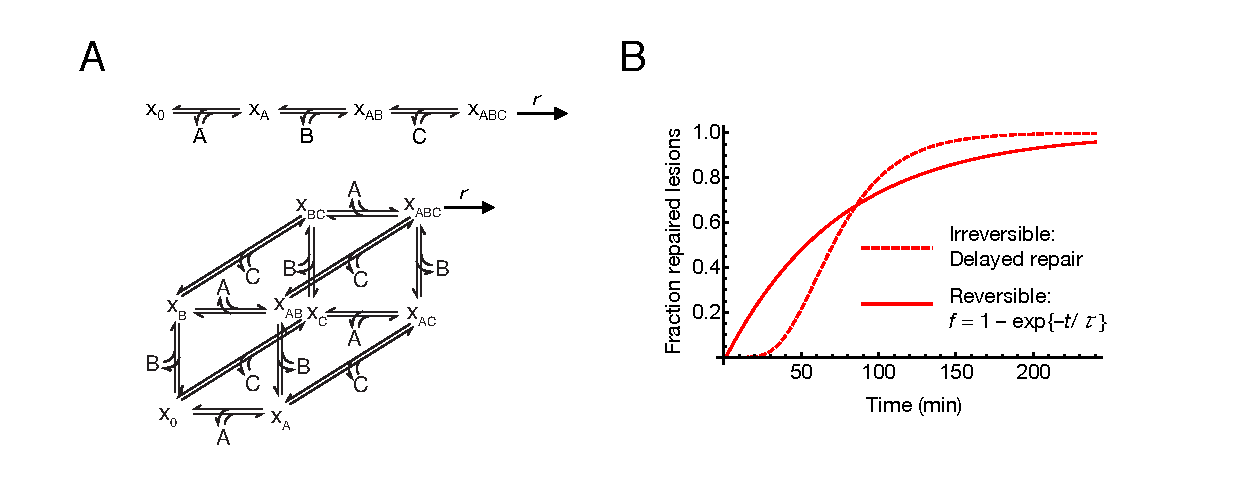
\includegraphics[width=1\textwidth]{Abbildungen/figure2_5_2.pdf}
\caption{\textbf{Simplified analytical model of the repair complex formation.} A) Sequential (upper panel) and random (lower panel) assembly scheme of the repair factors A, B and C to the DNA template $\text{x}_i$, $i \in \{\text{A, B, C, AB, AC, BC, ABC}\}$. $\text{x}_0$ denotes the empty lesion (e.g. damaged DNA). When the complex is fully assembled ($\text{x}_{\text{ABC}}$) it performs a catalytic repair step with rate $r$. B) Simulated repair time courses for random reversible (solid line) and irreversible (dashed line) repair factor assembly. For reversible binding ($k=l= \text{1 min}^{-1}, N=\text{9}$) the trajectory fits a mono-exponential repair kinetic with time constant $\tau$, whereas for irreversible binding the fit has sigmoidal shape ($l=\text{0}, k=\text{0.037 min}^{-1}, N=\text{9}$, chosen to get the same time constant). (Simulations by G. Terstiege \cite{Terstiege2010})}
\label{fig:reactionTiming}
\end{center}
\end{figure}


\section{Model structure and parametrization}
To examine the relation between rapid repair factor exchange and the slow first-order reaction kinetic, we extended the previously performed analysis \cite{Luijsterburg2010,Terstiege2010}, by considering a more realistic NER model. Conceptually, the model developed here, follows on the model introduced by Luijsterburg \textit{et al.} (2010) \cite{Luijsterburg2010}. In their model NER factors bind transiently to DNA repair intermediates to form catalytic complexes that, if complete, perform the next repair step. The latter are usually irreversible reactions embodying the sequential characteristic of this pathway (\textit{cf.}\ Figure \ref{fig:introScheme}A).\\
The nature of these repair intermediates has been widely investigated \textit{in vitro} and \textit{in vivo} \cite{Evans1997a,Mu1996,Polo2006,Tapias2004}.
The evolved model, presented here, distinguishes five DNA repair intermediates: damaged DNA, unwound DNA, incised DNA, resynthesised DNA and rechromatinised DNA. The molecular state of these intermediates defines the binding affinity for a specific set of repair proteins (\textit{cf.}\ Figure \ref{fig:ModelStructure}). Table \ref{tab:modelassumptions} summarizes all repair intermediates and lists the corresponding repair factors that show affinity for a particular repair intermediate. Repair factors that catalyse the enzymatic reaction if assembled are indicated. As stated before, FLIP measurements indicated that diffusion is not rate limiting for protein binding and therefore, we do not include it in the model (\textit{cf.}\ Section \ref{subsec:AccuFlipExp} and \cite{Rademakers2003,Zotter2006}).              


\begin{figure}[b!]
\begin{center}
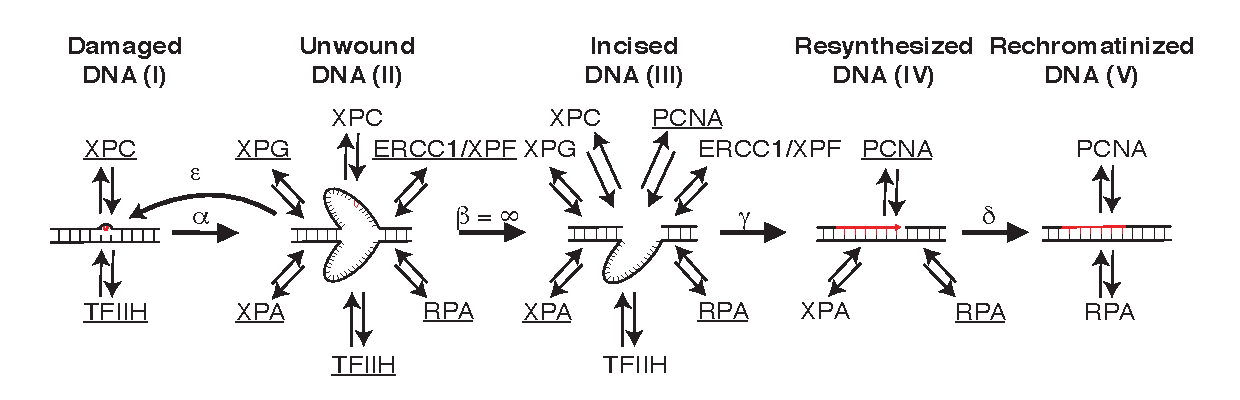
\includegraphics[width=1\textwidth]{Abbildungen/figure2_5.pdf}
\caption{\textbf{Schematic model description of the DNA repair mechanism.} The model distinguishes five individual repair intermediates: Damaged (I), unwound (II), incised (III), resynthesised (IV) and rechromatinised DNA (V). As indicated, specific tuples of repair proteins bind reversibly to the intermediates. Catalytic reactions, denoted by Greek letters, occur when the catalytic reaction complex (underlined proteins) is assembled.}
\label{fig:ModelStructure}
\end{center}
\end{figure}


Theoretical results suggest that the detection of damaged DNA sites by a single element instead of multiple elements simultaneously is crucial for the efficient initiation of the repair process \cite{Politi2005,Volker2001}. Within the NER pathway this prominent role is played by the lesion recognition factor XPC. Besides this experimentally verified exception, we assumed random and non-cooperative binding for all NER factors.\\ 
\begin{table}[t!]
	\small{
		\begin{tabular}{cccccc}
			\hline
			\rule{0pt}{2ex}
			\textbf{Repair}&\textbf{Binding} &	\textbf{Catalysed  process}&\textbf{Remarks}  	&\textbf{Ref.} \\ 
			\textbf{intermediate}&	\textbf{proteins} &	\textbf{Required proteins}&	& \\ \hline
			\rule{0pt}{3ex}
			(I) Damaged DNA&	XPC,TFIIH 	&Unwinding &Initiation by binding	&\cite{Evans1997a}
			\\ 
			&	(3 states)& (reaction $\alpha$)&  of XPC and subsequent &\cite{Riedl2003}\\
			&&XPC and TFIIH&	 recruitment of TFIIH. &\cite{Yokoi:2000:J-Biol-Chem:10734143}\\ 
			&&&&\cite{Rademakers2003}\\ 
			&&&& \cite{Volker2001} \\ 
			&&&&\\\hline
			\rule{0pt}{3ex}
			(II) Unwound DNA&XPC,TFIIH,&Dual incision &If the DNA becomes &\cite{Evans1997a} \\
			& XPG, XPA,&(reaction $\beta$)&devoid of any protein,&\cite{ODonovan:1994:Nature:8090225}\\
			&ERCC1/XPF,&TFIIH,XPG,&it will re-anneal (reaction &\cite{Sijbers:1996:Cell:8797827}\\
			&  RPA& XPA,  RPA&$\varepsilon$). Dual incision requires&\cite{Winkler2001}\\
			&(64 states)&and ERCC1/XPF&the endonucleases XPG& \cite{deLaat:1998:Genes-Dev:9716411}\\
			&&&  and ERCC1/XPF and is&\\
			&&&stimulated by TFIIH, &\\
			&&&XPA, RPA and possibly &\\
			&&&XPC.&\\
			&&&& \\ \hline
			\rule{0pt}{3ex}
			(III) Incised DNA &XPC,TFIIH,&Repair-synthesis&PCNA binds to the free&\cite{Evans1997a}\\
			& XPG, XPA,& (reaction $\gamma$)&3'-OH group generated by&\cite{Winkler2001}\\
			& ERCC1/XPF,&XPA, RPA and&  the ERCC1/XPF incision.&\\
			&RPA, PCNA& PCNA& DNA polymerase is also&\\
			&(128 states)&& required (not measured).	&\\
			&&&& \\   \hline
			\rule{0pt}{3ex}
			(IV) Resynthesised&XPA, RPA,&Rechroma-&Accumulation&\cite{Moser2005}\\
			DNA&	 PCNA& tinization& data imply that XPA&  \cite{Shivji:1995:Biochemistry:7711023}\\
			&(8 states)&(reaction $\delta$)& binds  to repaired DNA &\cite{Luijsterburg2010}\\
			&&RPA and PCNA&while the pre-incision &\\
			&&&	  proteins do not &\\
			&&& (Figure \ref{fig:accuImage}C).&\\
			&&&& \\ \hline
			\rule{0pt}{3ex}
			(V) Rechromatin- &RPA, PCNA &&RPA and PCNA associate&\cite{Riedl2003}\\
			ised DNA &(4 states)	&&with repaired intermediate V,&\cite{Luijsterburg2010}\\
			&&&as levels of bound eGFP-&\\
			&&&PCNA and eGFP-RPA&\\ 
			&&& are  high up to at least 4 h&\\
			&&& after UV irradiation, while&\\
			&&& other repair proteins are&\\   
			&&& no longer bound.&\\   &&&& \\ \hline
		\end{tabular}}
		\caption{\textbf{Model assumptions.} Adapted from Terstiege \textit{et al.} (2010) \cite{Terstiege2010}}\label{tab:modelassumptions}
	\end{table}
	\newpage
	\cleardoublepage  
	 
The model structure introduced above and shown in Figure \ref{fig:ModelStructure} was translated into an ordinary differential equation (ODE) system assuming mass-action kinetics for all protein-DNA interaction processes. Each equation describes the concentration of a single DNA state $y_{\pi}^{R}$ (\textit{cf.}\ Eqn. \ref{eqn:DNAstatesModel}) associated with a specific repair intermediate $R$ = I, II,\dots,V (damaged (I), unwound (II), incised (III), resynthesised (IV), rechromatinised (V)). The index $\pi$ represents a binary vector, where each position displays the presence or absence of a repair protein $p$ ($p$ $\in$ {C, T, G, A, F, R, P}, where XPC (C), TFIIH (T), XPG (G), XPA (A), ERCC1/XPF (F), RPA (R) and PCNA (P)). $\pi(p)=1$ if protein p is bound and $\pi(p)=0$ if not. The length of $\pi(p)$ is defined according to the model structure (\textit{cf.}\ Table \ref{tab:modelassumptions}) with: $\pi_{R=I} = \{ \text{C,T} \}$; $\pi_{R=II} = \{ \text{C,T,G,A,F,R} \}$; $\pi_{R=III} = \{ \text{C,T,G,A,F,R,P} \}$; $\pi_{R=IV} = \{ \text{A,R,P} \}$; $\pi_{R=V} = \{ \text{R,P} \}$. The time course of this model is described by

\begin{equation}\label{eqn:DNAstatesModel}
\frac{d}{dt}\;y_{\pi}^{R} =\sum_{p\text{ in }R}\eta \, \left( (-1)^{\pi(p)} \,l_{p}^{ R}\, y_{\pi}^{R}\left. \right|_{\pi(p)=1}+  \, (-1)^{1+\pi(p)}\, k_{p}^{ R} \,C_p(t)\,y_{\pi}^{R}\left. \right|_{\pi(p)=0}\right ) +E(y_{\pi}^{R}),
\end{equation}\\
where $\eta$ represents a cooperativity ensuring the inclusion of all cooperative binding events:

\begin{align*}
\eta =\left\{
\begin{array}{llll}
& 0 \quad   &\text{if}& R=\text{I} ~\wedge~ p=\text{C} ~\wedge~ \text{T}=1, \\
&     && R=\text{I} ~\wedge~ p=\text{T} ~\wedge~ \text{C}=0,\\
& 1 \quad &\text{otherwise}.&
\end{array}
\right.
\end{align*}
  
The kinetics describing protein exchange at the repair intermediates are characterized by the binding $k_{p}^{ R}$ and dissociation constants $l_{p}^{ R}$, respectively. The free protein concentrations are denoted by $C_p(t)$ representing seven additional ordinary differential equations for $p \in \{\text{C,T,G,A,F,R,P}\}$:

\begin{eqnarray}\label{Eqn:concentration}
\frac{d}{dt}\;C_p&=&\,r\left(\sum_{R=\text{I}}^{\text{V}} \sum_{\pi} \xi \left( \,\delta_{\pi (p)1}\;l_{p}^{ R}\, y_{\pi}^{R}- \,\delta_{\pi (p)0}\; k_{p}^{ R} \,C_p\,y_{\pi}^{R}\right)\right)
\end{eqnarray}  

Analogous to $\eta$, $\xi$ governs the sequential binding of XPC and TFIIH by:

\begin{align*}
\xi =\left\{
\begin{array}{l l ll}
& 0 \quad   &\text{if} & R=\text{I} ~\wedge~ \text{C}=0 ~\wedge~ \text{T}=1, \\
&    && R=\text{I} ~\wedge~ p=\text{C} ~\wedge~ \text{C}=\text{T}=1, \\
&    &&R=\text{I} ~\wedge~ p=\text{T} ~\wedge~ \text{C}=\text{T}=0, \\
& 1 \quad& \text{otherwise}.&
\end{array}
\right.
\end{align*}

The Kronecker delta 
 \begin{align*}
\delta_{ij}=\left\{
\begin{array}{l l l l}
&1 \quad   &\text{if} & i=j\\
&0 \quad& \text{if } & i \neq j\\
\end{array}
\right.
\end{align*}
ensures that a protein only binds to complexes, where it is yet missing and only leaves complexes, where it is actually present. The factor $r$ takes account of the volume ratio of the local damage to nuclear volume, which was estimated as 0.1 (\textit{cf.}\ Section \ref{sec:LD_volume}).\\
Finally, when an enzymatic complex has fully assembled at the DNA template, it catalyses the next repair step, which is represented in the model by the term $E(y_{\pi}^{R})$ in Eqn.\ \ref{eqn:DNAstatesModel}. After damage recognition by XPC, damaged DNA is unwound by the helicase TFIIH with the unwinding activity $\alpha$, whereas XPC acts as a stabilizing/proof-reading factor in parallel. Accordingly, $E(y_{\pi}^{R})$ translates into the following catalytic reactions for damaged DNA ($R= \text{I}$):
$$E(y_{00}^\text{I})=\;\varepsilon\;y_{000000}^\text{II} \quad \text{ and }\quad
E(y_{11}^\text{I})=\;-\alpha \;y_{11}^\text{I}.$$
If all proteins fall off the DNA template due to false damage detection, the DNA will re-anneal with the rate $\epsilon$. Otherwise a complex formed by TFIIH, XPG, XPA, XPF and RPA will eventually promote the excision of the lesion DNA strand leading to the following catalytic reactions for unwound DNA ($R= \text{II}$): 	
\begin{align*}
	\begin{array}{l l l}
		E(y_{000000}^\text{II})&=&-\;	\varepsilon	\;y_{000000}^\text{II}\;, \\ E(y_{110000}^\text{II})&=&\;	\alpha	\;y_{11}^\text{I} 	\text{ and }\\
	    E(y_{011111}^\text{II})&=&-\	\beta	\;y_{011111}^\text{II}.
	\end{array}
\end{align*}

Once the lesion strand is excised with incision rate $\beta$, the remaining repair steps are irreversible. Incised DNA is resynthesised with the rate $\gamma$ by the resynthesis complex  XPA-RPA-PCNA. XPA is assumed to assemble at post-incision repair intermediates as suggested by experiments with inhibited incision that showed accelerated dissociation FLIP kinetics for XPA  \cite{Luijsterburg2010}. This result is supported by a chromatin immunoprecipitation (ChIP) \label{par:schip} experiment with antibodies against XRCC1-Lig III showing the co-precipitation of XPA and RPA but not XPC and TFIIH \cite{Moser:2007:Mol-Cell:17643379}. Evidence for the importance of PCNA and RPA for the resynthesis reaction was shown by Shivji \textit{et al.} \cite{Shivji:1995:Biochemistry:7711023}, and therefore we incorporate the following catalytic reactions for incised DNA ($R= \text{III}$):  
            
\begin{align*}
\begin{array}{l l llll}
E(y_{1111111}^\text{III})&=&\;	\beta \;	y_{011111}^\text{II}	 \quad \text{and}
&E(y_{0001011}^\text{III})=&\;	-\gamma	\;y_{0001011}^\text{III}.	 \\
\end{array}
\end{align*}

In correspondence to the previously described accumulation measurements (\textit{cf.}\ Figure \ref{fig:accuImage}), only RPA and PCNA stay bound during chromatin remodelling (the last modelled repair intermediate). This leads to the following enzymatic reactions for resynthesised DNA  ($R= \text{IV}$) and rechromatinised DNA ($R= \text{IV}$):


\begin{align*}
\begin{array}{l l llll}
E(y_{111}^\text{IV})&=&\;	\gamma \;	y_{0001011}^\text{III},\\	 
E(y_{011}^\text{IV})&=&\;	-\delta	\;y_{011}^\text{IV} \text{ and }	 \\
 E(y_{11}^\text{V})&=&\;	\delta	\;y_{011}^\text{IV}.
\end{array}
\end{align*}

Due to the non-cooperativity assumption of all NER factors, there are a total of $\text{2}^N$ repair states where $N$ denotes the number of repair proteins assembling to the particular repair intermediate. The only exception is the sequential assembly of TFIIH, after lesion detection by XPC, which reduces the number of states for damaged DNA to $\text{2}^\text{2}$-1 = 3 states. For the remaining repair intermediates we derive  $\text{2}^\text{6}$ = 64 states for unwound DNA;  $\text{2}^\text{7}$ = 128 states for incised DNA; $\text{2}^\text{3}$ = 8 states for resynthesised DNA and $\text{2}^\text{2}$ = 4 states for rechromatinised DNA. This results in a total of 214 states including seven differential equations for the free NER-factor protein concentrations. \\
Summing over all repair states and the respective intermediates associated to one repair factor, we can simulate its accumulation kinetic. The initial conditions are the measured free protein concentrations denoted in Table \ref{tab:nuclearconcentrations}\cite{Terstiege2010,Luijsterburg2010} and the initial amount of inflicted damages was estimated with  $y_{00}^{\text{I}}$ = 3.33 \textmu M \cite{Verbruggen2014}. The remaining initial states were assumed to be zero. To reproduce the FLIP kinetic for a specific repair factor, all corresponding dissociation constants were set to zero when the FLIP experiment started (at the time where protein accumulation at LD reached the plateau level). Accordingly, FLIP kinetics were acquired after 600 s for XPC and ERCCC1/XPF, 900 s for XPG and TFIIH, 2000 s for XPA and 7200 s for PCNA. 


 

\section{A maximum likelihood approach for efficient model fitting}
\label{sec:maximumLL}
To find a realistic parametrisation for the temporal development of the repair states $y_\pi^R$ (\textit{cf.}\ Eqn.\ \ref{eqn:DNAstatesModel}) the model was mapped to $m$ observables $z_k$ via the function $f_{z_k}$:

  \begin{equation}
  	z_k(t_i,\theta) = f_{z_k}(t_i,y(t_i,\theta),\theta).
  	\label{eqn:observable}
  \end{equation} 

The observables $z_k$ are parametrised by $\theta$ and resemble experimentally-derived quantities at time $t_i$. $\theta$ depicts binding, dissociation and catalytic constants. Each model observable $z_k(t_i,\theta)$ corresponds to the measured data $z_k^\dag(t_i)$ with intrinsic noise $\epsilon_{ki}$. The data is usually the sum of measurement noise combined with the naturally occurring biological variability. Assuming additive, normally distributed noise leads to $z_k^\dag(t_i) = z_k(t_i,\theta) + \epsilon_{ki}$ with $\epsilon_{ki} \sim N(0,\sigma_{ki}^2)$. To calibrate the measured data $z_k^\dag(t_i)$ with the model observables $z_k(t_i,\theta)+\epsilon_{ki}$, we applied a maximum likelihood approach as distance measure which translates, considering normally distributed noise, into:
\begin{equation}
\label{eqn:likelihood}
L(z_k^\dag \textbar \theta) = \prod_{k=1}^m \prod_{i=1}^{d_k} \frac{1}{\sqrt{2\pi \sigma_{ki}^2}}\exp \left( -\frac{1}{2\sigma_{ki}^2}\left(z_{ki}^\dag(t_i) - z_k(t_i,\theta)\right)^2\right).
\end{equation}
  
Here, $d_k$ denotes the number of distinct experimental data-sets ($t_i,z_k^\dag$) for each measured observable $k = 1,\ldots,m$, measured at the time points $t_i$ with $i = 1,\ldots,d_k$. $\sigma_{ki}^2$ are the variance components of the measurement noise of each data point. Instead of maximizing the likelihood it is equivalent and numerically more efficient to minimize its negative logarithm multiplied with 2: $-2\log(L(z_k^\dag\textbar\theta))$, which we will refer to in the following as $\chi^{2}$.  

\begin{equation}\label{eqn:chiSquare}
\chi_\theta^2 = -2\log(L(z_k^\dag\textbar\theta)).
\end{equation}

For the minimization of $\chi^{2}$ the choice for $\theta$ is controlled by $\sigma_{ki}^2$ (\textit{cf.}\ Eqn.\ \ref{eqn:likelihood}). As shown by Raue and colleagues \cite{Raue2013}, for a reliable estimation of the model parameters $\theta$, the simultaneous approximation of $\sigma_{ki}^2$ together with the model dynamics leads to a statistically more accurate assessment of the model parameters than using noise estimations from preprocessed data \cite{Raue2013}. Accordingly $\sigma_{ki}^2$ can be considered as parametrised function

\begin{equation}
\sigma_{k}(t_i,\theta) = f_{\sigma_{k}}(t_i,z_(t_i,\theta),\theta),
\end{equation}    

wherein additional parameters are introduced representing the type and magnitude of the modelled noise. Analogous we applied an additive error model for each observable with the parametrised function $\sigma_{k}(t_i,\theta) = s_a$ and $\epsilon_{ki} \sim N(0,\sigma_{ki}^2)$, where $s_a$ is included in $\theta$.\\ 
For reasons of fitting-speed efficiency we implemented our model into the online-available D2D software environment \cite{Raue2013} optimized for MATLAB (2011a, The Mathworks Inc., Natick, MA). The integrated fitting procedure applies the trust region algorithm LSQNONLIN, which is pre-implemented in MATLAB. The algorithm requires the derivatives of the objective function with respect to the parameters (\textit{cf.}\ Eqn.\ \ref{eqn:likelihood}). The inner derivatives $dy(t,\theta)/d\theta$, also called sensitivities, provide gradient information about the parameter landscape and thus, are crucial to guide the optimization algorithm to the nearest optimum. The sensitivities can be passed into the form of sensitivity equations 

\begin{equation}
	\frac{d}{dt}\frac{dy(t,\theta)}{d\theta} = \frac{\partial f_y}{\partial y}\frac{dy(t,\theta)}{d\theta}+\frac{\partial f_y}{\partial \theta},
\end{equation}  

which represent additional ordinary differential equations (ODEs) \label{sec:ODE} that are solved in parallel to the original ODE system (\textit{cf.}\ Eqn.\ \ref{eqn:DNAstatesModel} and Eqn.\ \ref{Eqn:concentration})\cite{Leis1988}. Applying sensitivity equations instead of a simple finite difference approximation proved to be numerically more accurate and computationally faster \cite{Raue2013}. Both, model and sensitivity ODEs were solved with the CVODES algorithm written in ANSI \label{sec:ANSI} standard C \cite{Hindmarsh2005}. \\
To avoid terminating the optimization procedure in a local minimum we used a 'multi-start' approach by drawing the initial parameter vector using Latin hypercube sampling (LHS) \cite{Owen2014}. In contrast to a random sampling approach, LHS provides a better coverage of the sampling space by maximizing the distance between successive parameter drawings \cite{Raue2013}.    

\newpage



\section{NER model fits accumulation, FLIP and repair synthesis measurements}    

To derive faithful fitting results we reiterated the optimization process 250 times. For each iteration the starting parameters were redrawn by Latin hypercube sampling. Despite the size of the model, with respect to data points and the number of parameters, the majority of fits terminated within one order of magnitude compared to the global $\chi^{2}$ minimum (\textit{cf.}\ Figure \ref{fig:LHS}).
\begin{figure}[b!]
	\begin{center}
		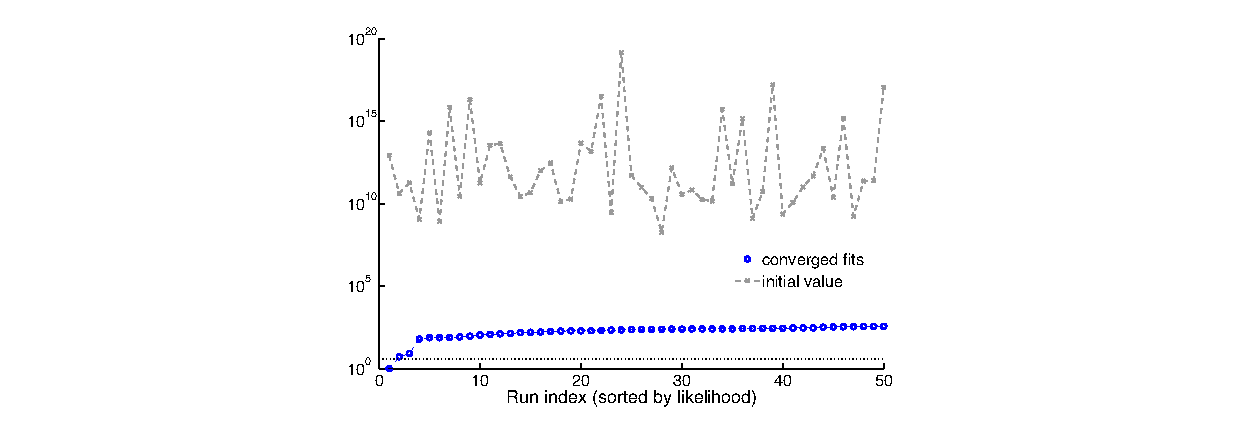
\includegraphics[width=1\textwidth]{Abbildungen/figure2_6_4.pdf}
		\caption{\textbf{Parameter estimation for the 50 best fits after initial Latin hypercube sampling.} Visualization of performance using the 50 (out of 250) best independent optimization runs (blue dots depict final optima of each individual run). Initial guesses (grey stars) were generated by Latin hypercube sampling. For illustrative purposes the global optimum is centred to 1.}
		\label{fig:LHS}
	\end{center}
\end{figure} 

Compared to the average initial $\chi^{2}$-value, the average fit improvement was about eight orders of magnitude. For the optimal parameter set, the model fits the experimental data comprising accumulation, FLIP, perturbation and repair synthesis measurements (\textit{cf.}\ Figure \ref{fig:ModelFit_accu_flip}A, B, C; estimated measurement errors are shown as shaded area around the fit). The accumulation kinetics (\textit{cf.}\ Figure \ref{fig:ModelFit_accu_flip}A) are depicted as concentrations scaled by the volume of the locally damaged area (\textit{cf.} Eqn.\ \ref{Eqn:concentration}), which were estimated with 10\% \label{sec:LD_volume} of the nuclear volume (average derived from segmentation results of the nucleus and the LD foci). We believe that this specification is more intuitively comprehensible  compared to scaling by the whole nuclear volume as performed by Luijsterburg \textit{et al.}\cite{Luijsterburg2010}. It allows the realistic comparison between simulated and measured microscopy images of NER factor accumulation and EdU incorporation (\textit{cf.}\ Figure \ref{fig:Fitt_accu_Mic}).  

\begin{figure}[htbp]
	\begin{center}
		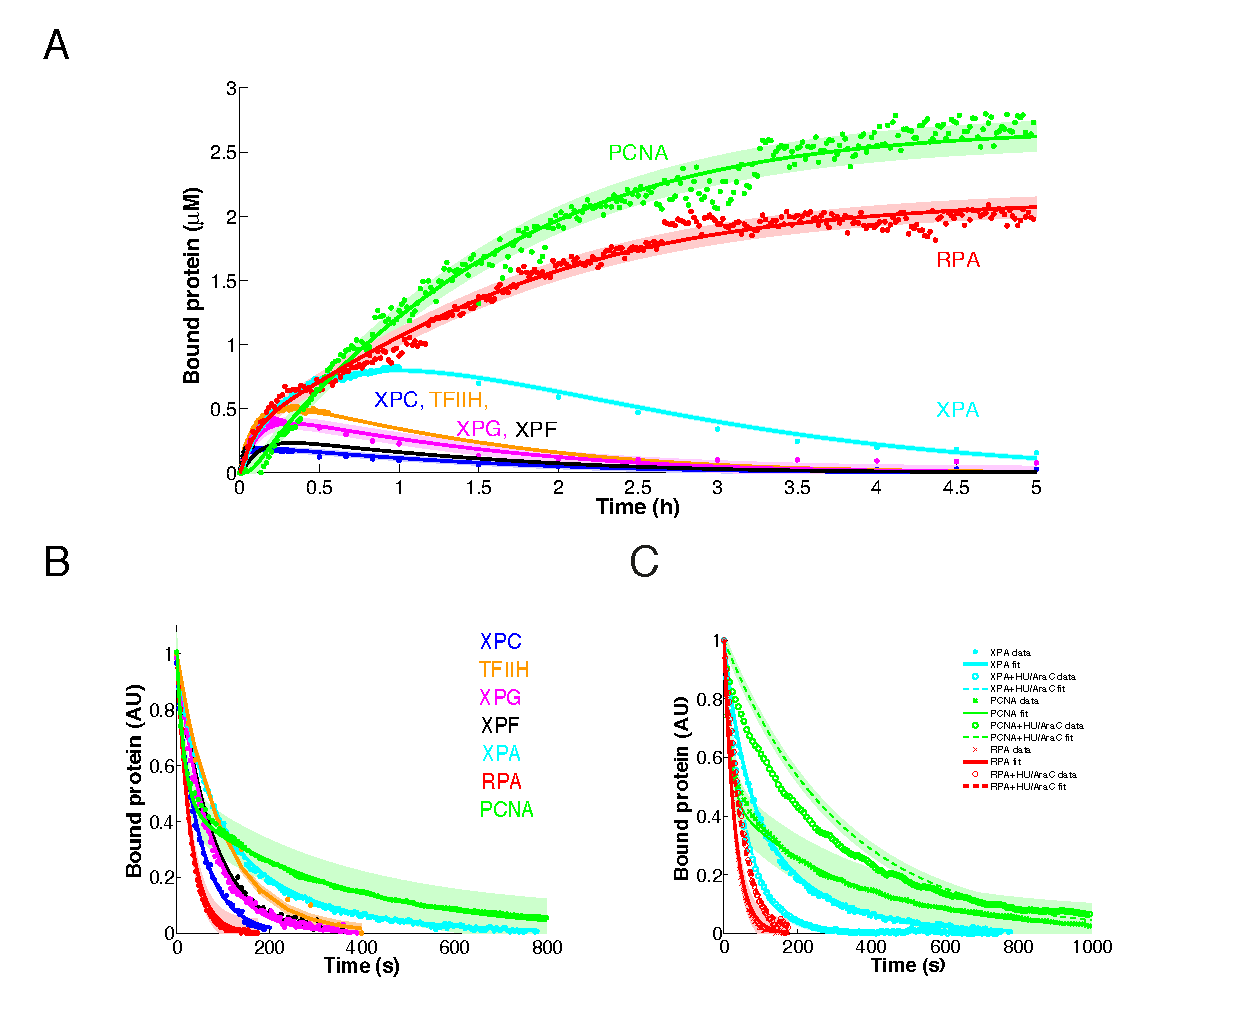
\includegraphics[width=1\textwidth]{Abbildungen/figure2_6.pdf}
		\caption{\textbf{Quantitative NER model fits to accumulation and dissociation time courses.} A) and B) Simulation (lines) and measurement (dots) of the accumulation and dissociation kinetics for the repair factors XPC, TFIIH, XPG, XPA, XPF, RPA and PCNA. Estimated errors are depicted as shaded area. C) Fitted FLIP time courses of XPA, RPA and PCNA in the absence or presence of AraC and HU on locally irradiated cells. (Experiments by M. Luijsterburg)}
		\label{fig:ModelFit_accu_flip}
	\end{center}
\end{figure}
\begin{figure}[t!]
\begin{center}
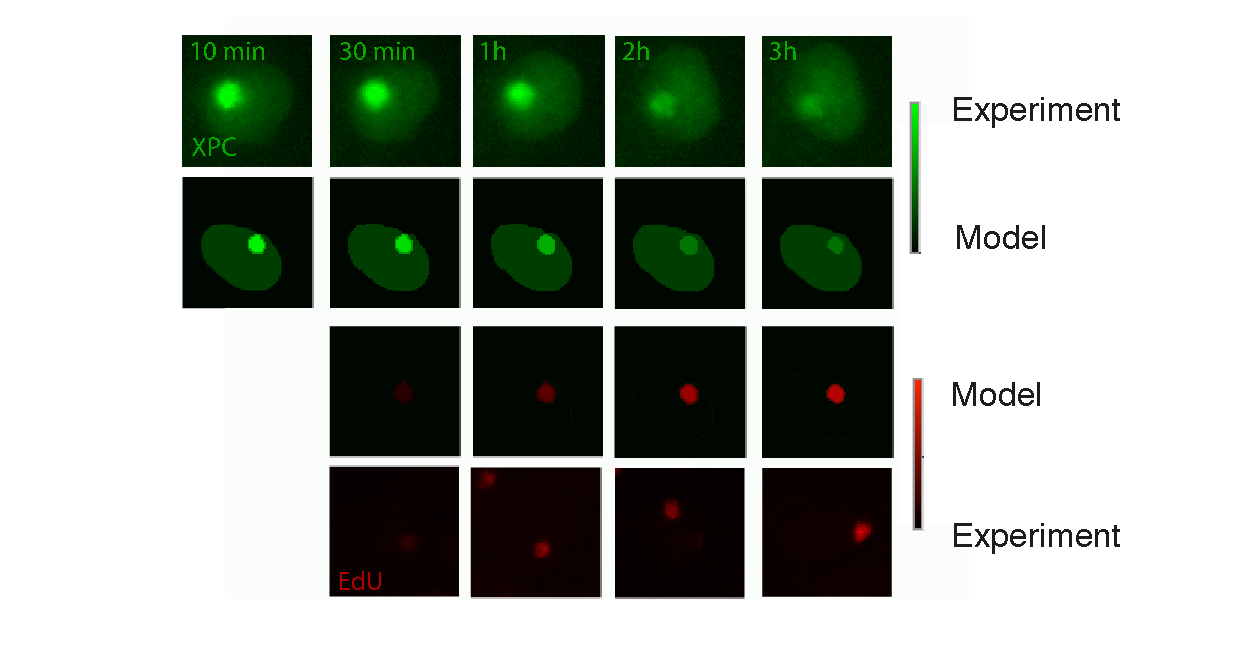
\includegraphics[width=1\textwidth]{Abbildungen/figure2_6_2.pdf}
\caption{\textbf{Comparison between measured and simulated single cell microscopy images.} Simulated time courses and the associated microscopy images for GFP tagged XPC (two upper rows) and EdU incorporation (two lower rows). Simulated XPC expression intensities were normalized to the nuclear intensities of the microscopy images. For the EdU incorporation intensities were scaled according to the highest and lowest intensity values of the microscopy images. (Experiments by P. Verbruggen)}
\label{fig:Fitt_accu_Mic}
\end{center}
\end{figure}

\section{Profile likelihood analysis identifies realistic model of NER}
\label{sec:identifiabilityAnalysis}
In this section we quantify the quality of the model fit and determine whether the current model structure is competent for reliable predictions concerning experimentally unobserved system behaviour. This capability depends on the structural and practical identifiability of the model, which can be influenced by functionally related parameters or by the limited amount and quality of the data, respectively \cite{Cobelli1980,Swameye2003}. Both can be analysed and tested numerically by a formalism called profile likelihood estimation (PLE)\label{sec:PLE}\cite{Venzon1988,Murphy2000,Raue2009}, where the multi-dimensional model uncertainty inflicted by an individual parameter is projected to a one-dimensional profile likelihood (PL)
\begin{equation}
PL(\theta_i) = \max_{\forall j \neq i} [L(z_k^\dag \lvert \theta_j)].
\label{eqn:PL} 
\end{equation}
One parameter $\theta_l$ with $l\in\{{1,\ldots,N}\}$ at a time, is gradually fixed along this dimension for different values of $p$. In each step the negative log-likelihood $\chi_{\theta_l}^2(p)$ is minimized (\textit{cf.}\ Eqn.\ \ref{eqn:chiSquare}), fitting all other parameters $\theta_k$ with $k\in\{{1,\ldots,N}\}$; $k\neq l$. Subsequently, the identifiability of a parameter $\theta_l$ can be determined by $\Delta \chi_{\theta_l}^2(p)$, which describes the difference between the parameter dependent local minimum $\chi_{\theta_l}^2(p)$ and the global $\chi^{2}$ minimum
\begin{eqnarray}
	\Delta \chi_{\theta_l}^2(p) &=& \min_{\{\theta_k\textbar k=1,\ldots,N;k\neq l\}} \left( \chi^{2} (\theta_1,\ldots,\theta_{l-1},p,\theta_{l+1},\ldots,\theta_N )\right)\nonumber \\
	&-& \quad \! \min_{\{\theta_k\textbar k=1,\ldots,N\}} \quad \!\! \left( \chi^{2} (\theta_1,\ldots,\theta_N )\right).
\end{eqnarray}  

Confidence bounds for the particular parameter depend on the threshold $Q_{\chi^{2}}(1-a,df)$, which represents the $(1-a)$ quantile of the $\chi^{2}$-distribution with $df$ degrees of freedom. The associated point-wise confidence intervals are defined as
\begin{equation}
CI_{1-a}^{\theta_l}= \{p\textbar \Delta \chi_{\theta_l}^2(p)\leq Q_{\chi^{2}}(1-a,1)\}.
\label{eqn:confidenceIntervals}
\end{equation} 

For one fixed parameter at a time and thus one degree of freedom we can derive the common confidence region $CI_{95\%}$, which corresponds to a $\chi^{2}$-distribution quantile of $Q_{\chi^{2}}(95\%,1)$ = 3.8. A parameter $\theta_l$ is identifiable, if the confidence interval $CI_{1-a}(\theta_l)$ is finite, which can be determined directly from the graph of the profile likelihood $\Delta \chi_{\theta_l}^2(p)$ for different values of $p$ (\textit{cf.}\ Figure \ref{fig:profileLikilihoods}).\\ 
We applied the identifiability analysis on our NER model (\textit{cf.}\ Eqn.\ \ref{eqn:DNAstatesModel} and Eqn.\ \ref{Eqn:concentration}) comprising 40 binding and dissociation parameters and 4 catalytic reaction constants. However, only under the assumption that the repair factor exchange at unwound and incised DNA is equal (\textit{cf.}\ Figure \ref{fig:PLE_NER_overview} with the exception of PCNA) all binding and dissociation constants were identifiable. The same holds true for the dissociation kinetics of TFIIH from damaged and unwound DNA. This reduces the number of fitted parameters to 14 binding, 13 dissociation and 4 catalytic rate constants.
\begin{figure}[htbp]
	\begin{center}
		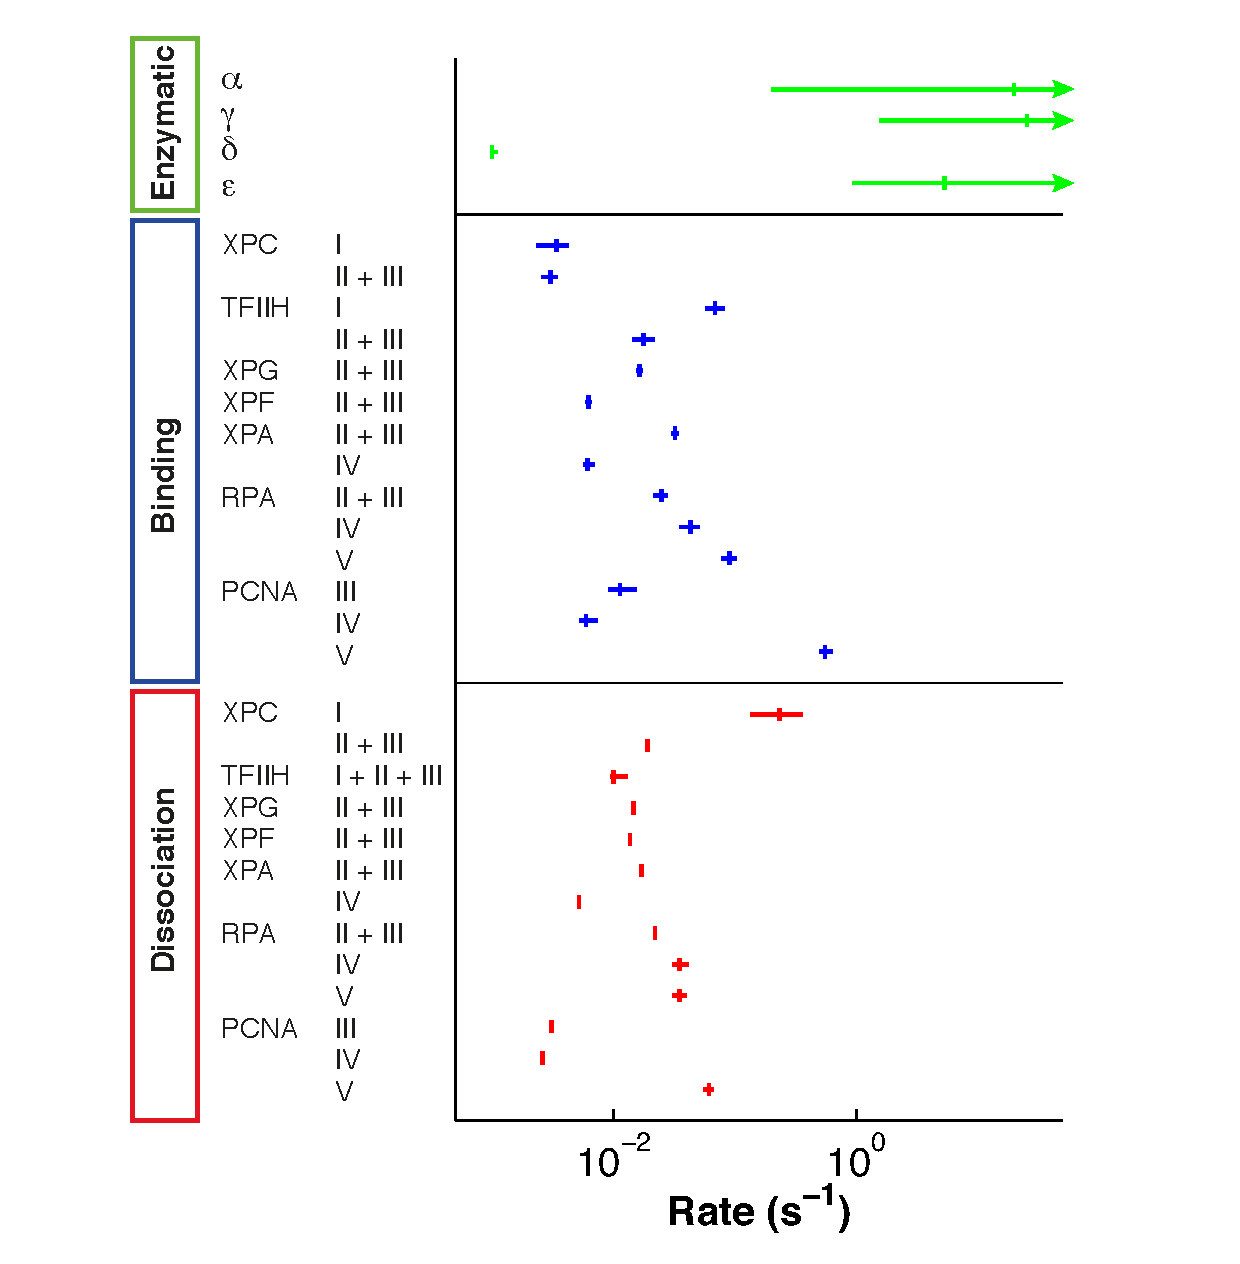
\includegraphics[width=1\textwidth]{Abbildungen/figure2_9.pdf}
		\caption{\textbf{Parametrisation identifies realistic model for NER.} Mean values (vertical bars) and confidence intervals (horizontal bars) of catalytic (green), binding (blue) and dissociation constants (red) characterizing the dynamic assembly of NER factors at the successive repair intermediates (damaged DNA I, unwound DNA II, incised DNA III, resynthesised DNA IV, rechromatinised DNA V). Arrow heads indicate infinite confidence intervals.}
		\label{fig:PLE_NER_overview}
	\end{center}
\end{figure}

Besides the slow rate of rechromatinisation $\delta$, presumably identifiable due to the slow decrease in accumulated XPA (\textit{cf.}\ Figure \ref{fig:ModelFit_accu_flip}), all catalytic rates are fast. This is seen by the existence of lower bounds on the rate constants of the order of 1 $\text{s}^{-\text{1}}$. For the numerical values of the parameters see Table \ref{tab:parameter_bigTable} and Table \ref{tab:parameter_catalyticRates}. 



\begin{landscape}
	\centering
\begin{table}[t]
	
	\small{
	\begin{tabular}[angle=90]{p{2cm}ccccccc}
	\hline
	\textbf{Value}    & \textbf{ XPC} & \textbf{TFIIH} & \textbf{XPG} & \textbf{XPF} & \textbf{XPA} & \textbf{RPA} & \textbf{PCNA}  \\
	\hline
	\multicolumn{8}{l}{\textbf{Damaged DNA}} \\
	$\text{K}_{\text{d}}$({\textmu}$\text{M})$                                                  & 9.35                & 0.052 & NA &NA&NA&NA&NA     \\
	& (3.46;16.09)     &(0.044;0.072)  &&&&&   \\
	\multicolumn{8}{l}{\textbf{Unwound DNA}} \\
	$\text{K}_{\text{d}}$({\textmu}$\text{M})$                                                  & 0.864                     & 0.204                   & 0.395                 &2.446                 &0.147                    &1.222                    &NA     \\
	& (0.635;1.006)     & (0.163;0.259)             & (0.373;0.419)		&(2.344; 2.596)&(0.138;0.158)     &  (1.048;1.36)  &   \\
	\multicolumn{8}{l}{\textbf{Incised DNA}} \\
	$\text{K}_{\text{d}}$({\textmu}$\text{M})$                                                  & 0.864                     & 0.204                   & 0.395                 &2.446                 &0.147                    &1.222                    &0.388     \\
	& (0.635;1.006)     & (0.163;0.259)             & (0.373;0.419)		&(2.344; 2.596)&(0.138;0.158)     &  (1.048;1.36) 	 & (0.319;0.538)  \\
	\multicolumn{8}{l}{\textbf{Resynthesised DNA}} \\
	$\text{K}_{\text{d}}$({\textmu}$\text{M})$                                                  & NA                          &NA                         & NA                      &NA                      &0.236                   &1.167                    &0.605     \\
	&                               &                              &                           &                          &(0.222;0.27)     &  (0.924;1.521)  & (0.531;0.747)  \\
	\multicolumn{8}{l}{\textbf{Rechromatinised DNA}} \\
	$\text{K}_{\text{d}}$({\textmu}$\text{M})$                                                  & NA                          &NA                         & NA                      &NA                      &NA                         &0.538                    &0.154     \\
	&                               &                              &                           &                          &                            &  (0.438;0.645)  & (0.134;0.182)  \\
	\hline
\end{tabular}}

\begin{adjustwidth}{-3.5 cm}{}
\captionsetup{width=1.24\textwidth}
\caption{\textbf{$\text{K}_{\text{d}}$Values.} NA, not applicable. $\text{K}_{\text{d}}$ ($k_{\text{off}}/k_{\text{on}}$) values are given for every repair protein and arranged in columns. Reference parameter set and 95\% confidence intervals (in parentheses) are shown.}\label{tab:KdValues}
\end{adjustwidth}
\end{table}

\end{landscape}

The $\text{K}_{\text{d}}$ values ($k_{\text{off}}/k_{\text{on}}$), depicting the protein binding affinities to the respective DNA repair intermediate fall into a physiological realistic range between $\sim$100 nM and $\sim$1 \textmu M (\textit{cf.}\ Table \ref{tab:KdValues}). Only XPC has a particular low affinity of 9 \textmu M, which is consistent with previous findings reporting that the time until DNA incision is mainly determined by the slow lesion recognition \cite{Luijsterburg2010}.\\        
Having an identifiable model allows us to make more precise computational predictions. For example, we can simulate the unobservable fraction of incised DNA (\textit{cf.}\ Figure \ref{fig:ModelFit_intermed}, green trajectory). As the EdU incorporation measurement shows, the damaged (blue) and repaired (red) DNA kinetics are tightly coupled. This omits a higher accumulation of incised DNA.\\ 


In summary, for the development of a realistic model of the DNA repair pathway we integrated live-cell imaging data of the assembly and dissociation kinetics of all core NER factors and linked it directly to the DNA repair kinetics. The extended dataset identifies a total of 31 model parameters including 14 binding, 13 dissociation and 4 catalytic rate constants. Therefore, quantitative predictions with the model on the functioning of NER are no longer limited by parameter non-identifiability.  

\begin{figure}[htbp]
	\begin{center}
		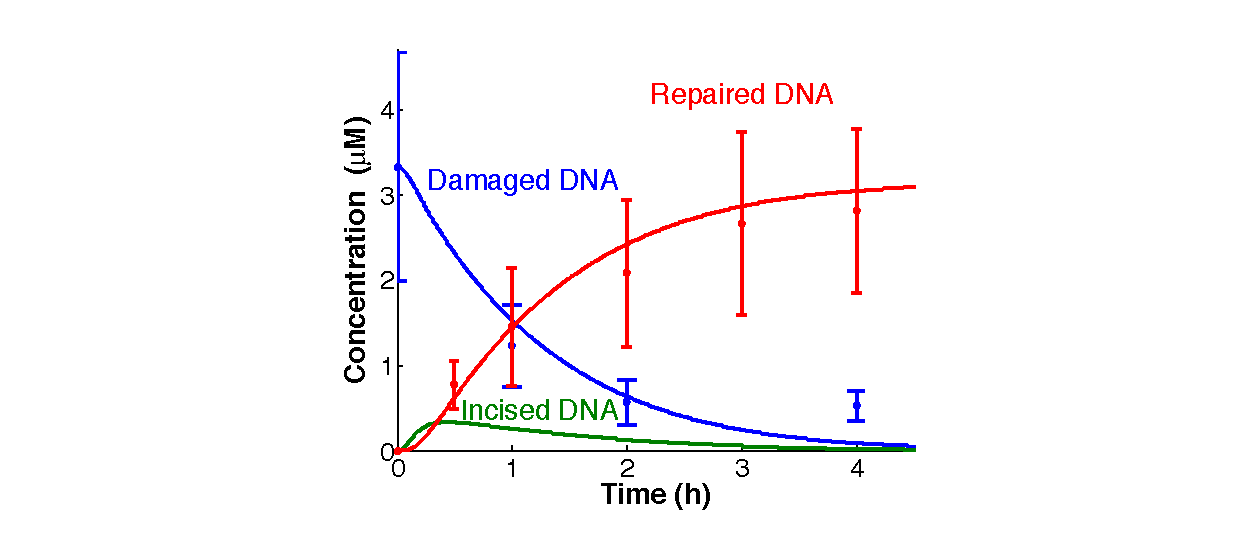
\includegraphics[width=1\textwidth]{Abbildungen/figure2_7.pdf}
		\caption{\textbf{Short delay between DNA damage removal and DNA repair synthesis omits accumulation of incised DNA.} Experimental (dots with error bars) and simulated (lines) time courses for damaged DNA (blue) and DNA repair synthesis (red). Simulated trajectories depict repair intermediate I+II for damaged DNA and repair intermediate IV+V for repaired DNA (\textit{cf.}\ Figure \ref{fig:ModelStructure}). Model prediction for incised DNA (green) constitutes from DNA repair intermediate III. (Experiments by P. Verbruggen)}
		\label{fig:ModelFit_intermed}
	\end{center}
\end{figure}

